\documentclass[a4paper,11pt]{article}

%\usepackage[latin1]{inputenc}
\usepackage[utf-8]{inputenc}
\usepackage{hyperref}
\usepackage{graphicx}
%\usepackage{url}

%% Macros
\def\haskell{\texttt{Haskell}}

%%%%%%%%%%%%%%%%%% Inicio do Documento %%%%%%%%%%%%%%%%%
\begin{document} % TENTAR POR RODAPE E/OU CABECALHO E ESPAÇOS NO INICIO DE CADA PARÁGRAFO

\title{Ha\_CWB - Haskell Concurrency Workbench, sort of ...}
\author{José Manuel Serra Marques (35839) \and Carlos Manuel Gomes Vilhena (35812)\and \emph{Departamento de Informática :: Universidade do Minho}}
\date{\today}
\maketitle

%  Resumo inicial
%Peq Resumo
\begin{abstract}
Para a criação do Haskell Concurrency Workbench HA\_CWB foi necessário dividir esse projecto em duas fases: \\

\begin{itemize}
\item Animação de processos através de grafos de transição - nesta fase, no âmbito da disciplina de Métodos de Programação 4 e principal 
objectivo para o projecto da mesma disciplina, foram definidos processos em Haskell, e um conjunto de módulos também em Haskell para a 
manipulação de processos (concretamente avaliação de processos) e criação de grafos de tansição.
\item Cálculo de processos - segunda fase do projecto, ainda não abordada, que visa a interacção entre processos, a criação de digramas de 
sincronização de processos, bem como verificar Bissimulação e Equivalência Estrita, Equivalência Observacional e Igualdade de Processos. Para 
além disso, será ainda objectivo do projecto incluir um \textit{parser} para a linguagem \textit{$\Pi$-Calculus}. \\
Nesta fase, será ainda incluído um modo gráfico, para facilmente a ferramenta poder ser usada. O modo gráfico será criado em \textit{WX-Haskell}, 
e toda a ferramenta criada estará por de trás do motor gráfico.
\end{itemize}

\end{abstract}

\newpage

% Indice				%ja esta
\tableofcontents

% objectivos & Mote

%%% Local Variables: 
%%% mode: latex
%%% TeX-master: "main"
%%% End: 

\section{Objectivos}
Nesta secção vamos falar um pouco sobre a razão que nos levou a lançar este projecto também iremos abordar mais detelhadamente  os objectivos que temos para o nosso trabalho.\\
A ideia deste pojecto, surgiu-nos quando foi propos-to na disciplina de MP4 a utilização de uma excelente ferramenta (\textsf{CWB}) que visa a animação de processos e a formulação de vários tipo de provas sobre os mesmos. Mas apesar de ser uma boa ferramenta, tem o grande defeito de ser muito difícil (para não dizer impossível) de instalar. Para ajudar ainda mais, existe na Universidade do Minho uma grande cultura para a utilização da poderosa linguagem de programação \haskell, e foi então que nos surgiu a ideia da construção de uma ferramenta em \haskell permitindo assim tirar todas as vantagens desta linguagem de programação.\\
Passando agora mais concretamente aos nossos objectivos que temos para este projecto, é nosso ``sonho'' que a nossa ferramenta tenha pelo menos as mesmas funcionalidades do \textsf{CWB}, com uma interface um pouco mais polida e ainda adicionar mais funcionalidade ao nível da interação do utilizador com o resultado da computação realizada sobre a lista de processos inicial.\\
Actualmente a ferramenta lê de um ficheiro, um conjunto de processos inicial e depois de seleccionado oo processo pelo qual deseja iniciar, é gerado o grafo de transições desse processo para um limite desejado, sendo de seguida esse resultado exportado para um ficheiro \texttt{GraphViz}. O  \texttt{GraphViz} foi escolhido como forma de mostrar o resultado pois é muito simples a geração da representação do grafo de transições de precessos arbitrariamente complexos, sendo também muito fácil a visualização por parte do utilizador do respectivo resultado.\\
Como objectivos futuros, ou seja, funcionalidades para próximas versões da ferramenta, estamos empenhados em adicionar o reconhecimento da linguagem de {\textsf{CCS}} com anotação bem como a possibilidade da realização de tarefas bem mais interessantes sobre os processos como sejam a prova de simulações, bi-simulações, equivalências observacionais, etc.

% FIM  %Trofa

% software utilizado  %Trofa		%ja esta
\section{Software Utilizado}
Aqui vamos enunciar as três principais ferramentas de software utilizadas no desenvolvimento do trabalho. Na última secção falaremos resumindamente de outras ferramentas que nos ajudaram a levar o trabalho a ``bom porto''.  \\
Como compilador principal da linguagem \haskell, utilizamos a ferramenta \textsf{GHC}. \\
Na construção do interpretador de ficheiros utilizamos a ferramenta \textsf{Alex} como \textit{lexer} e a ferramenta \textsf{Happy} como gerador do \textit{parser}.\\
O \textsf{Alex} gera a lista de \textit{tokens} reconhecidos no texto de entrada e o \textsf{Happy} interpreta esses \textit{tokens} de acordo com a linguagem especificada.

\subsection{GHC}
A ferramenta \textsf{GHC} foi escolhida para este trabalho pois ela pemite-nos compilar o trabalho e não apenas interpreta-lo. Isto é tanto ao mais importante pois é nosso objectivo gerar uma ferramenta autónoma e não apenas desenvolver um conjunto de bibliotecas para serem posteriormente interpretadas num qualquer interpretador de \haskell.\\
Assim sendo, na fase de desenvolvimento do trabalho utilizamos o interpretador \textsf{GHCi}, o que nos permitiu ir monitorizando e corrigindo os erros e quando quisemos gerar a ferramenta \textbf{hacwb} usamos o compilador \textsf{GHC}.\\
Mais informações em \url{http://www.haskell.org/ghc/}.

\subsection{Alex}
A ferramenta \textsf{Alex} pretende ser um gerador de analisadores léxicos para a linguagem {\haskell} em que cada \textit{token} é descrito sobe a forma de expressão regular. A melhor maneira de a descrever é dizer que \textsf{Alex} está para o {\haskell} como o \textsf{Flex} está para o \texttt{C/C++}.\\
Mais informações em \url{http://www.haskell.org/alex/}.

\subsection{Happy}
\textsf{Happy} pretende ser gerador de \textit{parsers} também para a linguagem \haskell, ou seja, dada uma determinada linguagem na forma \textbf{BNF} (Backus–Naur form), o \textsf{Happy} constroi o respectivo \textit{parser}. A melhor maneira para o descrever é dizer que o \textsf{Happy} está para o {\haskell} como o \textsf{YACC/Bison} está para o \texttt{C/C++}.\\
De seguida apresenta-se a linguagem utilizada no para este trabalho e as respectivas acções semânticas.
\newpage
\begin{verbatim}
Root :: { LstProcesses String }
Root : PROCNAME '=' Process ';' Root  { ($1, $3):$5 }
     | {- empty -} { [] }

Process :: {  Process String }
Process : Rests Proc_Body { if $1==[] then $2 else (New $1 $2) }
     | {- empty -} { Zero }

Rests :: { [String] }
Rests : NEW '{' More_Rests '}' { $3 }
      | {- empty -} { [] }
More_Rests : ACT ',' More_Rests { $1:$3 }
           | ACT { [$1] }

Proc_Body :: { Process String }
Proc_Body : Pro '+' Pro { Or $1 $3 }
        | Pro '|' Pro { Paralel $1 $3 } 
        | Pro { $1 }
Pro : Pro_Complex { $1 }
    | P { $1 }
Pro_Complex : '(' Proc_Body ')'{ $2 }
P : ACT '.' P { Dot (Var $1) $3 }
  | '~' ACT '.' P { Dot (Comp $2) $4 }
  | '0' { Zero }
  | PROCNAME {NameP $1}
\end{verbatim}

De notar que a cada produção da gramática está associada a respectiva acção semântica. Como se pode ver acima, o resultado final é a lista de processos contidos no ficheiro de entrada, no tipo de dados que utilizamos no nosso trabalho.\\
Mais informações em \url{http://www.haskell.org/happy/}.

\subsection{Outras}
Outra ferramenta que utilizamos no nosso trabalho foi a \textsf{Make} que vem com todas as distribuições \texttt{Unix}, permitindo desta forma automatizar o processo de criação da ferramenta. Para isso basta apenas fazer ``make hacwb'' e o executável é gerado automáticamente.

	
% Hacwb					%ja esta
\section{HaCWB}

Nesta secção, será explicado o objectivo desta ferramenta, bem como o modo de utilização. Todas 
as opções permitidas serão explicadas, bem como o modo de funcionamento.

\subsection{Descrição da Ferramenta}

Como já foi dito anteriormente, neste momento esta ferramenta apenas manipula processos e permite 
criar grafos de transição. Assim, recebendo como parâmetro de entrada um ficheiro em CCS contendo 
processos, o \textit{parser} lê-os, e coloca-os numa estrutura de dados intermédia, mais concretamente, 
uma lista de pares da forma (Nome do Processo , Processo), para posterior manipulação.

\subsection{Utilização do HaCWB}

Para melhor compreender e utilizar o hacwb, passamos à descrição de todas as opções disponíveis, e 
ainda o seu modo de funcionamento. Serão apresentados ainda alguns breves exemplos de utilização.

\begin{itemize}
\item \textit{-h} - Opção de ajuda. Quando incluida nas opções, é imprimido um texto de ajuda, com 
todas as opções da ferramenta.\\
Segue-se um exemplo da invocação da ferramenta com esta opção:\\
\begin{verbatim}
/src/bin$ ./hacwb -h

HaCWB - A Haskell tool to manipulate processes.
Usage: hacwb options ...

List of options:

  -H, -h                    --help           
                           output a brief help message
  -L file_in, -l file_in    --load=file_in   
                           specify input file
  -S file_out, -s file_out  --save=file_out  
                           save transition graph
  -G, -g                    --graph          
                           generate transition graph
  -F, -f                    --save           
                           generate multiple files 
                           with transition graphs


For more information see README file.
\end{verbatim}
\item \textit{-g} - Para criar grafos de transição a partir de um ficheiro de \textit{input}, é necessário 
incluir esta opção na ferramenta.
\item \textit{-l} - Esta opção requer argumento. Assim, dado um ficheiro de entrada em CCS, o hacwb 
faz o \textit{parsing} do ficheiro, e grava para uma estrutura de dados intermédia os processos lidos.\\
Para invocar o hacwb com esta opção: \textit{hacwb -g -l"fin"}.\\
Note-se que invocando desta maneira o hacwb, todo o \textit{output} será redireccionado para o monitor.\\
De seguida, mostra-se um exemplo de um ficheiro de \textit{input}, aceite pelo hacwb:\\
\begin{verbatim}
P1 = (c.d.0 + w.0);

P2 = new {a} (a.0 | ~a.b.0);
\end{verbatim}
\item \textit{-s} - Para guardar os grafos de transição criados apenas num ficheiro, basta invocar a ferramenta 
com esta opção seguida de um argumento (nome do ficheiro de saída sem extenção), para que todos os grafos de 
transição possam ser guardados (codificados em GraphViz), para posteriormente o utilizador vizualizar.\\
Para invocar o hacwb com esta opção: \textit{hacwb -g -l"fin" -s"fout"}.\\
Após invocar o hacwb com o ficheiro de entrada referido no ponto anterior, e depois de gerar o respectivo 
\textit{postscript} através da ferramenta \textit{dot} incluida no GraphViz, obtemos os seguintes grafos de 
transição:

\begin{figure}[!htb]
\begin{center}
\label{fig:tg}
\resizebox{.35\textwidth}{!}{\includegraphics{out.ps}}
\caption{Grafo de transição referente ao ficheiro de entrada apresentado anteriormente.}
\end{center}
\end{figure}

\item \textit{-f} - Por fim, para guardar cada processo lido do ficheiro de entrada independentemente, utiliza-se 
a opção -f. Desta forma, sao criados \textit{n} ficheiros (com \textit{n} número de processos, e em que o nome 
do ficheiro é o inteiro respectivo).\\
Para invocar o hacwb com esta opção: \textit{hacwb -g -l"fin" -f}.\\
O resultado desta invocação, para i ficheiro de entrada anterior, são 4 ficheiros \textit{dot}, com os grafos de 
transição separados por ficheiros.
\end{itemize}

\subsection{Estruturas de dados criadas para definir Processos}

Aqui, apresentam-se as estruturas de dados mais importantes criadas ao longo da realização deste trabalho prático, 
para definir processos e grafos de transição.\\
Em primeiro ligar é necessário definir processos. Para isso foi criado o tipo \textit{Process}, com todos os construtores 
necessários. Um desses construtores, mais concretamente o consrutor \textit{NameP}, foi criado para dar um nome a um processo, 
para assim permitir que processos de invoquem mutuamente. Segue-se o tipo de dados:\\

\begin{verbatim}
data Process a = Or (Process a)  (Process a)
                | Paralel (Process a) (Process a)
                | Dot (Action a) (Process a)
                | Zero 
                | New [a] (Process a)
                | NameP String
\end{verbatim}

Depois de definir processos, torna-se necessário definir Acções. Tomamos como acções a acção de sincronização \textit{Tau}, 
bem como as variáveis e os seus complementares:\\

\begin{verbatim}
data Action a = Var a 
                | Comp a 
                | Tau
\end{verbatim}

Quando lêmos um ficheiro de entrada, gravamos o conteúdo do ficheiro CCS numa estrutura intermédia, chamada \textit{LstProcesses}, 
definida mais a baixo, para atribuir a cada processo um nome:\\

\begin{verbatim}
type LstProcesses a = [(String, Process a)]
\end{verbatim}

Por fim, para definir grafos de transição foi definido um tipo de dados, similar a \textit{Rose Tree}, contendo no nodo 
o processo e de seguida uma lista de todas as possíveis derivações:\\

\begin{verbatim}
data TransG a p = Node p [(a,TransG a p)]
\end{verbatim}

Para além destas estruturas de dados, foram criadas mais estruturas auxiliares, das quais destacamos a estrutura de estado, 
utilizada na avaliação de processos (possívelmente infinitos):\\

\begin{verbatim}
type Stt a = (Int, Path a, LstTrees a)
\end{verbatim}

Em que:\\

\begin{verbatim}
type Path a = [(Action a, Process a)]

type LstTrees a = [(Process a, Path a)]
\end{verbatim}



% Modulos HaCWB				%nao da tempo
\include{ModulosHaCWB}

% TODO					%ja esta
\section{TODO}

Para que o Haskell Concurrency Workbench esteja finalizado, é necessário ainda desenvolver alguns pontos. 
Segue-se uma lista resumida do trabalho futuro proposto:
\begin{itemize}
\item Melhoramento a nível do código - Trata-se de um objectivo a curto prazo. Pretende-se melhorar o código criado, 
de forma a tornar os algoritmos mais eficientes de forma mais elegante.
\item Cálculo de Processos - trata-se da verdadeira essência do HaCWB. A introdução deste \textit{item} 
vai permitir a interacção de processos (criação de diagramas de sincronização) e ainda todo o tipo de verificações:
\begin{itemize}
\item Bissimulação e Equivalência Estrita;
\item Equivalência Observacional;
\item Igualdade de Processos.
\end{itemize}
\item Como já foi referido, será criado um \textit{parser} para \textit{$\Pi-Calculus$}, juntando-se assim ao 
parser de CCS.
\item Por fim, para facilitar a utilização desta ferramenta, será incluído um modo gráfico a ser construído utilizando 
a biblioteca \textit{WX-Haskell}.
\end{itemize}


% Conclusao  %Trofa

%%% Local Variables: 
%%% mode: latex
%%% TeX-master: "main"
%%% End: 

\section{Conclusão}
Chegamos à secção mais interessante do projecto que é aquela em que contamos a nossa experência no decorrer deste projecto.\\
A fase inicial foi um pouco estranha pois, como nenhum de nós tem muita experiência neste campo, a base do trabalho estava a mudar constantemente o que não nos permitia ter alguma coisa em concreto a funcionar. Depois a base do trabalho começou a estabilizar, permitindo assim começar a pensar mais estruturadamente o que contribui para que os  resultados começacem a aparecer o que começou a dar mais alento.\\
O desenvolvimento deste trabalho bem como a pesquisa de tecnologias associadas ao mesmo consumiu muito tempo, prolongando assim para a época de exames o que fez com que desacelerasse o seu desenvolvimento o que fez com que não fossem incluidas algumas funcionalidades (GUI, CSS anotado) mas que irão ser incluídas em versões futuras.\\
Para finalizar, resta dizer que foi muito interessante poder ``fazer'' alguma coisa mais com a teoria que aprendemos na aulas ao longo do semestre, funcionando como uma motivação extra. 


% bibliografia
\include{bibliografia}

\end{document}
